\chapter{System Design and Methodology} \label{chapter:3}

\section{Data Inputs}
The main data input to the propagation of satellites in this project is Two-Line Element sets (TLEs). TLEs are a common publicly accessible format which describes Earth-orbiting satellite positions. The primary source of TLE data is SpaceTrack \cite{spacetrack}. Although SpaceTrack is the primary source, many projects such as this project and other research rely on sources such as CelesTrak, which takes the data from SpaceTrack and organizes it into specific groupings \cite{celestrakTLE}. Some examples of these groupings are shown in Listing~\ref{list:satellite_categories}.

\begin{figure}[ht]
\centering
\begin{minipage}{0.6\linewidth}
\begin{itemize}
    \item \textbf{Starlink}
    \item \textbf{ISS}
    \item \textbf{Earth observation satellites}
    \item \textbf{Weather satellites}
    \item \textbf{Communications satellites}
    \item \textbf{Active vs.\ debris groupings}
\end{itemize}
\end{minipage}
\caption{Common satellite groupings provided by CelesTrak}
\label{list:satellite_categories}
\end{figure}

While other sites exist such as N2Y0 and AMSAT, CelesTrak remains one of the most reliable and widely used platforms due to consistent updates synchronized with SpaceTrack and curated categories which help simplify data access. CelesTrak updates the majority of its TLE files approximately every two hours. Its Starlink data can expect multiple updates per day, making it suitable for this project's application \cite{usradioguyNewTLE}.

\section{Two Line Element Data}
TLEs are a standardized format used to describe the orbital properties of Earth-orbiting satellites. A TLE represents a satellite's orbit at a specific moment in time, known as the epoch. Because the TLE format is simple and lightweight, it is widely supported and remains the most common method for distributing orbit data for tracking and prediction.

A TLE consists of three lines: line 0 (optional) contains the satellite name, line 1 contains identification and basic orbital parameters, and line 2 describes remaining orbital elements such as inclination. This is summarized in Table~\ref{tab:summaryOfTle}. An example of TLE data is shown in Listing~\ref{fig:tle-starlink-5694}.

\begin{figure}[ht]
\centering
\begin{verbatim}
STARLINK-5694
1 55481U 23015AJ  26041.24424508  .00002920  00000+0  23114-3 0  9992
2 55481  42.9978 128.2652 0001315 248.0292 112.0411 15.02536911166474
\end{verbatim}
\caption{Two-Line Element (TLE) for STARLINK-5694}
\label{fig:tle-starlink-5694}
\end{figure}

\begin{table}[ht]
\caption{Summary of key parameters in a Two-Line Element}
\centering
\small
\renewcommand{\arraystretch}{1.3}
\begin{tabular}{|l|l|p{7.5cm}|}
\hline
\textbf{Field} & \textbf{Value} & \textbf{Meaning} \\ \hline
Satellite Name & STARLINK-5694 & Human-readable satellite identifier \\ \hline
Catalog Number & 55481 & Unique NORAD satellite ID \\ \hline
Classification & U & Unclassified satellite \\ \hline
Launch Year & 2023 & Part of the International Designator (23) \\ \hline
Launch Number & 015 & 15th launch of the year 2023 \\ \hline
Launch Piece & AJ & Specific object from that launch \\ \hline
Epoch (Year) & 2026 & TLE epoch year (26) \\ \hline
Epoch (Day) & 41.24424508 & Day of year when the TLE is valid \\ \hline
Inclination (deg) & 42.9978 & Tilt of orbit relative to Earth's equator \\ \hline
Mean Motion (rev/day) & 15.02536911 & Orbits per day ($\approx$95.8 min period) \\ \hline
\end{tabular}
\label{tab:summaryOfTle}
\end{table}

\FloatBarrier

\section{Orbit Propagation}
TLE data describes a satellite's orbit at a specific moment in time, known as the epoch. To determine a given satellite's position at times throughout the simulation, an orbit propagation model is required. Orbit propagation uses the orbital parameters contained within the TLE along with a model for orbital perturbations to predict the satellite's future position and velocity as a given time stamp
 
In this project, the Simplified General Perturbations Model 4 (SGP4) \cite{vtSpacetrk} is used for orbit propagation. SGP4 is a widely used algorithm for propagating satellite orbits for organizations such as NORAD and NASA \cite{patt1994sgp4}. The model accounts for dominant perturbations which affect LEO satellites such as Earth's uneven gravitational field, and atmospheric drag. SGP4 is computationally efficient and provides sufficient accuracy for coverage estimation.

For each satellite, SGP4 computes a time varying state vector consisting of position and velocity in the True Equator Mean Equinox (TEME) frame. This allows the system to determine where each satellite is located at any given time during the simulation, which is essential for evaluating visibility and coverage. These are calculated at discrete time intervals defined by the simulation parameters, such as every 10 seconds, to balance accuracy and computational load.


\section{Coordinate Systems} \label{section:coordinateTransformations}
To determine satellite visibility and coverage, satellite orbits and ground user locations must be expressed in a common coordinate system. This allows for accurate calculations of line-of-sight and beam-width constraints. Different coordinate systems are used at different stages of the analysis, with each serving a distinct purpose in representing satellite motion or Earth fixed locations. This sections aims to introduce the coordinate systems used in this project and their roles in the methodology. The mathematical transformations between these coordinate systems will be discussed in section \ref{section:mathematical_coordinate_transformation}.

In this project, the satellites which are propagated using SGP4 are expressed in the True Equator Mean Equinox (TEME) frame, while ground sites are typically given in geodetic coordinates. It is therefore necessary to convert both to an Earth-Centered Earth-Fixed (ECEF) frame \cite{asteRisk2023, astropy:2022}. This provides a common reference frame for enable geometric calculations such as line-of-sight and beam-width evaluations.



\subsection{TEME}
TEME is the native output frame of SGP4. It is non-rotating with respect to Earth's surface and must be converted before comparison with geodetic locations. TEME is an Earth centered reference frame whose orientation is relative to Earth's equatorial plane and mean equinox. It is designed specifically for use with TLE data and the mathematical approximations which are employed in SGP4 \cite{asteRisk2023}.

TEME is well suited for representing satellite motion because it provides a stable reference for orbit prediction that is not fixed to the Earth's surface which rotates. However, as this coordinate system does not rotate with the Earth, positions expressed in this frame cannot be directly compared with ground locations which rotate with the Earth directly. 


\subsection{ECEF}
ECEF is a rotating Cartesian coordinate system which is fixed relative to the Earth's surface. It's origin is located at the Earth's center of mass, with axes aligned to the Earth's rotation and geographic geometry. As it rotates with the Earth, ECEF is ideal for representing ground locations.  ECEF is used to describe the observer's positions which come from latitude, longitude coordinates, and provides a common reference frame for evaluation relationships between satellites and ground locations. By expressing both the ground user and the satellite in ECEF, direct calculations such as line-of-sight and beam-width evaluations can be carried out \cite{Navipedia_CTRS_2011}. a Comparison between geodetic and ECEF coordinates is shown in Figure~\ref{fig:ECEF}

\begin{figure}[h!]
    \centering
    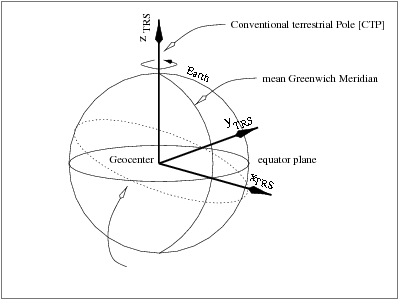
\includegraphics[width=0.4\textwidth]{figures/ECEF.png}
    \caption{ECEF Coordinate System \cite{mathworks_radar_coordinates}}
    \label{fig:ECEF}
\end{figure}

\FloatBarrier
\section{Assumptions}
To simplify the analysis and focus on the core aspects of satellite coverage, several assumptions are made in this project. These assumptions simplify the modelling process while preserving sufficient accuracy for the intended analysis. 

The first assumption is that the satellites are assumed to follow trajectories predicted by SGP4 when initialized with publicly available TLE data. While SGP4 accounts for things such as Earth's oblate shape and atmospheric drag, it does not capture all short term maneuvering. Satellites are assumed to follow the predicted trajectories without performing maneuvers such as station keeping or collision avoidance. 

The second assumption is that the Earth is modelled using a WGS-84 ellipsoid for all geodetic to ECEF transformations. Local terrain variation, orography, and surface irregularities  are not considered. Ground users are assumed to be at sea level unless otherwise specified, visibility issues due to terrain and other obstructions such as buildings or vegetation are not considered. A free-space path model loss model is instead implemented. Even with this free space path loss model, atmospheric effects such as rain, wind and any other weather related fading effects are not included in the analysis. There is a constant loss factor per unit of distance which is assumed. 

The third assumption is the antenna radiation patterns are simplified using a fixed half-power beam width model. Each satellite is assumed to have a single, ideal beam centered on its nadir direction, and beam forming, side-lobe effects, and other complexities of real antenna patterns are not considered. The beam width is assumed to be constant and does not vary with frequency or other factors. Beam-to-ground aligned is evaluated purely geometrically, based on angular separation without accounting for adaptive beam scheduling or multi-beam operation. To attempt to account for this a relatively wide beam width of 15 degrees is used, which is wider than the typical beam width of a LEO satellite, to provide a more conservative estimate of coverage.

The fourth assumption is that interference between satellites is modelled in a simplified manner. If multiple satellites are visible to a ground user at the same time, it is assumed that the satellite with the strongest signal (i.e., the smallest angular separation from the user's zenith) provides coverage, while others do not. Interference power is estimated by summing the reduced contributions of all visible satellites transmit power power based on a constant scalar.  

The fifth assumption is that handover dynamics are not explicitly modelled. WHen multiple satellites satisfy coverage criteria, the satellite which provides service is assumed to be the one with the best geometric alignment. Latency associated with handover, beam switching, and gateway routing is neglected. 

The sixth assumption is that user demand is assumed to be uniform across the coverage grid. Traffic load, contention between user, and scheduling policies, are outside the scope of this project. Throughput is modelled using the Shannon capacity formula to represent theoretical data rates. 

Finally, the analysis assumes that satellites are operate continuously and are always transmitting at their maximum power when they are visible. Satellite maintenance periods, power constraints, and operational outages are not considered.